\documentclass[12pt,letterpaper]{article}

\usepackage[T1]{fontenc}
\usepackage[utf8]{inputenc}
\usepackage[spanish,mexico,es-tabla,es-noshorthands]{babel}
\usepackage{newtxtext,newtxmath}          % Times New Roman
\usepackage[margin=2.5cm]{geometry}
\usepackage{graphicx}
\usepackage{float}
\usepackage{caption}
\usepackage{subcaption}
\usepackage{booktabs}
\usepackage{enumitem}
\usepackage{amsmath}          % no cargar amssymb: choca con \Bbbk de newtxmath
\usepackage{listings}
\usepackage{xcolor}
\usepackage{setspace}
\usepackage[colorlinks=true,allcolors=black]{hyperref}
\usepackage{todonotes}                    % usar [disable] para la versión final

\graphicspath{{evidencias/}{../assets/}}
\captionsetup{labelsep=colon,font=small,labelfont=bf}
\onehalfspacing
\setlength{\parskip}{6pt}

% Títulos de sección al estilo del formato de la profesora
\usepackage{titlesec}
\titleformat{\section}{\normalfont\large\bfseries}{}{0pt}{}
\titleformat{\subsection}{\normalfont\normalsize\bfseries}{}{0pt}{}

\definecolor{codekw}{RGB}{0,0,180}
\definecolor{codecm}{RGB}{0,128,0}
\definecolor{codestr}{RGB}{170,0,0}
\definecolor{codebg}{RGB}{248,248,248}

\lstdefinestyle{hdl}{
  language=VHDL,
  basicstyle=\ttfamily\footnotesize,
  keywordstyle=\color{codekw}\bfseries,
  commentstyle=\color{codecm}\itshape,
  stringstyle=\color{codestr},
  backgroundcolor=\color{codebg},
  numbers=left, numberstyle=\tiny\color{gray}, numbersep=8pt,
  frame=single, rulecolor=\color{gray!50},
  breaklines=true, breakatwhitespace=true,
  tabsize=2, showstringspaces=false, captionpos=b,
  extendedchars=true, inputencoding=utf8,
  literate={á}{{\'a}}1 {é}{{\'e}}1 {í}{{\'i}}1 {ó}{{\'o}}1 {ú}{{\'u}}1
           {Á}{{\'A}}1 {É}{{\'E}}1 {Í}{{\'I}}1 {Ó}{{\'O}}1 {Ú}{{\'U}}1
           {ñ}{{\~n}}1 {Ñ}{{\~N}}1 {ü}{{\"u}}1 {¿}{{?`}}1 {¡}{{!`}}1
}
\lstset{style=hdl}
\renewcommand{\lstlistingname}{Figura}   % el código se numera junto a las figuras


\usepackage{colortbl}
\definecolor{kgroupa}{RGB}{190,220,255}
\definecolor{kgroupb}{RGB}{255,224,178}

\begin{document}

\begin{titlepage}
\centering
\noindent
\begin{minipage}[c]{0.45\textwidth}\centering
  
\includegraphics[height=3.2cm]{logo-unam.jpg}
\end{minipage}\hfill
\begin{minipage}[c]{0.45\textwidth}\centering
  
\includegraphics[height=3.2cm]{logo-fi.png}
\end{minipage}

\vspace{1.2cm}
{\Large\bfseries UNIVERSIDAD NACIONAL AUTÓNOMA\\[2pt] DE MÉXICO\par}
\vspace{0.9cm}
{\large\bfseries FACULTAD DE INGENIERÍA\par}
\vspace{0.6cm}
{\large\bfseries INGENIERÍA EN COMPUTACIÓN\par}
\vspace{0.6cm}
{\bfseries Laboratorio de Organización de Arquitectura de Computadoras\par}
\vspace{0.9cm}
{\bfseries Reporte - Diseño de máquinas de estado\par}

\vspace{1.3cm}
\raggedright
{\bfseries NOMBRE DE LOS INTEGRANTES:}\\
Omar Alfonso Zendejas Labias \quad Grupo de Teoría: 04\\
Emiliano García Olvera \quad Grupo de Teoría: 02

\vspace{1.3cm}
{\bfseries NOMBRE DEL PROFESOR: ING. KAREN PÉREZ}

\vspace{0.6cm}
{\bfseries GRUPO: 06 \quad EQUIPO: 9}

\vspace{0.6cm}
{\bfseries SEMESTRE:} \underline{2027-1.}

\vspace{0.6cm}
\hfill {\bfseries FECHA DE ENTREGA: 15 de septiembre de 2026}
\thispagestyle{empty}
\end{titlepage}

\setcounter{page}{1}

\section{Objetivo}

Se busca analizar, diseñar e implementar una máquina de estados finitos a partir de una
carta ASM proporcionada, identificando el funcionamiento de los \textit{flip-flops} tipo
D como elementos de memoria. A partir del llenado de la tabla de transiciones y de la
reducción mediante mapas de Karnaugh se obtienen las funciones de estado siguiente y de
salida, las cuales posteriormente se implementan en VHDL y se verifican sobre la tarjeta
de desarrollo FPGA DE10-Lite.

\section{Introducción}

Una carta \textit{ASM} (\textit{Algorithmic State Machine}) es una representación
gráfica del comportamiento de un circuito secuencial, equivalente a un diagrama de
estados, en la que cada estado se dibuja como una caja rectangular y cada condición de
transición como una caja de decisión. A diferencia del diagrama de estados clásico, la
carta ASM se asemeja a un diagrama de flujo y resulta más directa para derivar, a partir
de ella, la tabla de transiciones del sistema.

En una implementación síncrona, el estado de la máquina se almacena en un conjunto de
\textit{flip-flops} tipo D, que actúan como elementos de memoria: en cada flanco de
\textit{clock} capturan el valor calculado como estado siguiente y lo mantienen hasta el
siguiente flanco. Las entradas $D$ de estos \textit{flip-flops}, así como las señales de
salida de la máquina, se obtienen como funciones booleanas del estado actual y de las
entradas del sistema; dichas funciones se simplifican mediante mapas de Karnaugh a
partir de la tabla de transiciones, siguiendo el procedimiento estándar de diseño de
circuitos secuenciales síncronos descrito, entre otros, por Savage Carmona \emph{et al.}
\cite{savage}.

\section{Desarrollo}

\subsection{Parte I. Análisis y diseño de la máquina de estados}

La carta ASM proporcionada para esta práctica se muestra en la figura
\ref{fig:asm}.

\begin{figure}[H]
  \centering
  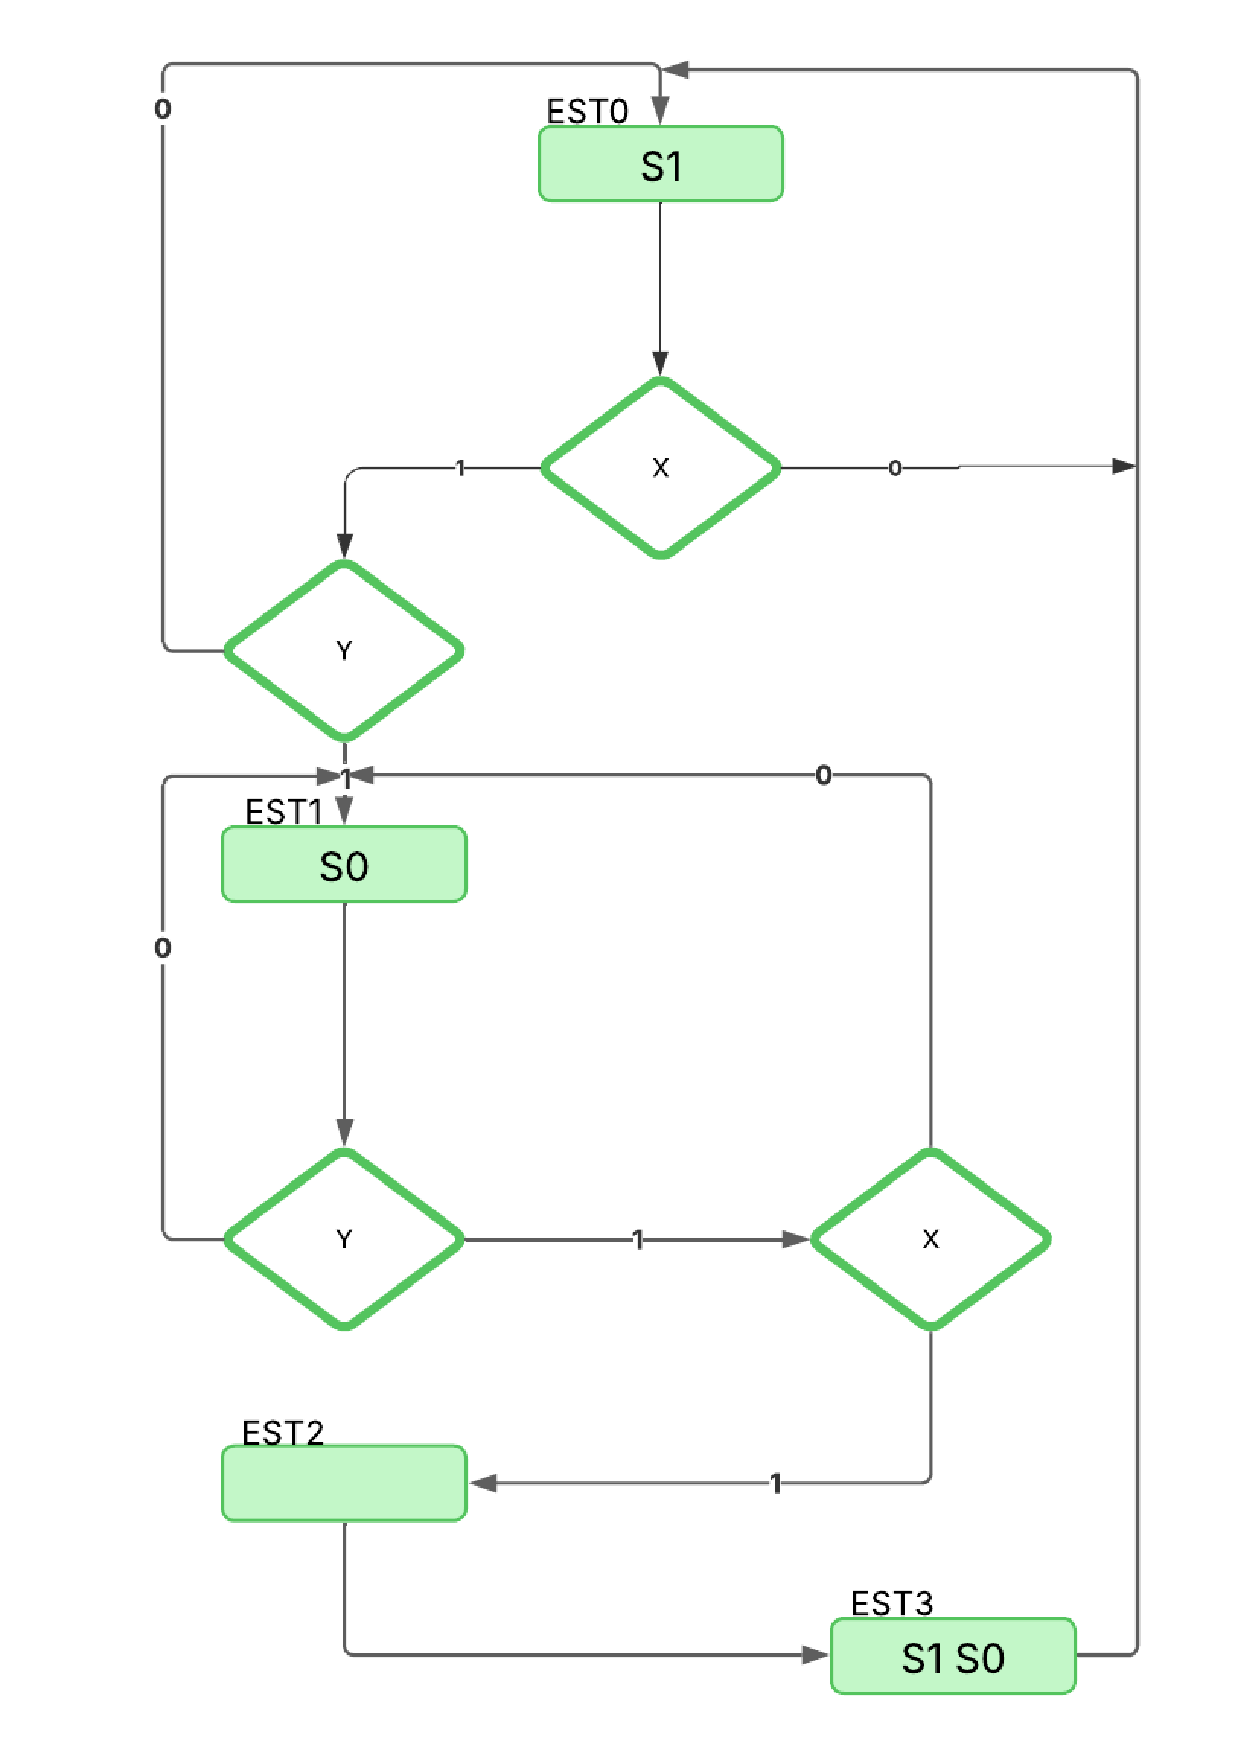
\includegraphics[width=0.55\textwidth]{Practica_2_ASM.pdf}
  \caption{Carta ASM del sistema, proporcionada en el manual de la práctica.}
  \label{fig:asm}
\end{figure}

\subsubsection{Identificación de estados, entradas y salidas}

La carta ASM define cuatro estados: EST0, EST1, EST2 y EST3. La máquina tiene dos
entradas, $X$ y $Y$, y dos señales de salida, $S_1$ y $S_0$, cuyo valor depende
únicamente del estado actual (es decir, se trata de una máquina de tipo Moore): EST0
activa $S_1$ ($S_1S_0=10$), EST1 activa $S_0$ ($01$), EST2 no activa ninguna salida
($00$) y EST3 activa ambas ($11$).

\subsubsection{Codificación de los estados}

Al ser cuatro estados se requieren 2 bits, almacenados en dos flip-flops tipo D con
salidas $Q_1Q_0$. Se propuso la codificación secuencial:
EST0$=00$, EST1$=01$, EST2$=10$, EST3$=11$.

\subsubsection{Tabla de transiciones}

Siguiendo las rutas de decisión de la carta ASM (figura \ref{fig:asm}) se obtiene la
siguiente tabla de transiciones, en la que un asterisco indica que la salida de ese
estado no depende de dicha entrada:

\begin{table}[H]
  \centering
  \begin{tabular}{cc|cc|cc|cc}
    \toprule
    \multicolumn{2}{c|}{Estado actual} & \multicolumn{2}{c|}{Entradas} &
    \multicolumn{2}{c|}{Estado siguiente} & \multicolumn{2}{c}{Salidas} \\
    Edo. & $Q_1Q_0$ & $X$ & $Y$ & Edo. & $Q_1Q_0$ & $S_1$ & $S_0$ \\
    \midrule
    EST0 & 00 & 0 & * & EST0 & 00 & 1 & 0 \\
    EST0 & 00 & 1 & 0 & EST0 & 00 & 1 & 0 \\
    EST0 & 00 & 1 & 1 & EST1 & 01 & 1 & 0 \\
    EST1 & 01 & * & 0 & EST1 & 01 & 0 & 1 \\
    EST1 & 01 & 0 & 1 & EST1 & 01 & 0 & 1 \\
    EST1 & 01 & 1 & 1 & EST2 & 10 & 0 & 1 \\
    EST2 & 10 & * & * & EST3 & 11 & 0 & 0 \\
    EST3 & 11 & * & * & EST0 & 00 & 1 & 1 \\
    \bottomrule
  \end{tabular}
  \caption{Tabla de transiciones obtenida a partir de la carta ASM.}
  \label{tab:transiciones}
\end{table}

\subsubsection{Mapas de Karnaugh}

A partir de la tabla \ref{tab:transiciones} se construyeron los mapas de Karnaugh de las
entradas $D_1$, $D_0$ de los flip-flops y de las salidas $S_1$, $S_0$, usando como ejes
$Q_1Q_0$ y $XY$:

\begin{figure}[H]
\centering
\begin{tabular}{cc}
\begin{tabular}{c|cccc}
 $Q_1Q_0\backslash XY$ & 00 & 01 & 11 & 10 \\
\hline
00 & 0 & 0 & 0 & 0 \\
01 & 0 & 0 & \cellcolor{kgroupb}1 & 0 \\
11 & 0 & 0 & 0 & 0 \\
10 & \cellcolor{kgroupa}1 & \cellcolor{kgroupa}1 & \cellcolor{kgroupa}1 & \cellcolor{kgroupa}1 \\
\end{tabular}
&
\begin{tabular}{c|cccc}
 $Q_1Q_0\backslash XY$ & 00 & 01 & 11 & 10 \\
\hline
00 & 0 & 0 & 1 & 0 \\
01 & 1 & 1 & 0 & 1 \\
11 & 0 & 0 & 0 & 0 \\
10 & 1 & 1 & 1 & 1 \\
\end{tabular}
\\[4pt]
$D_1$ & $D_0$ \\
\end{tabular}

\vspace{8pt}
\begin{tabular}{cc}
\begin{tabular}{c|cccc}
 $Q_1Q_0\backslash XY$ & 00 & 01 & 11 & 10 \\
\hline
00 & \cellcolor{kgroupa}1 & \cellcolor{kgroupa}1 & \cellcolor{kgroupa}1 & \cellcolor{kgroupa}1 \\
01 & 0 & 0 & 0 & 0 \\
11 & \cellcolor{kgroupb}1 & \cellcolor{kgroupb}1 & \cellcolor{kgroupb}1 & \cellcolor{kgroupb}1 \\
10 & 0 & 0 & 0 & 0 \\
\end{tabular}
&
\begin{tabular}{c|cccc}
 $Q_1Q_0\backslash XY$ & 00 & 01 & 11 & 10 \\
\hline
00 & 0 & 0 & 0 & 0 \\
01 & \cellcolor{kgroupa}1 & \cellcolor{kgroupa}1 & \cellcolor{kgroupa}1 & \cellcolor{kgroupa}1 \\
11 & \cellcolor{kgroupa}1 & \cellcolor{kgroupa}1 & \cellcolor{kgroupa}1 & \cellcolor{kgroupa}1 \\
10 & 0 & 0 & 0 & 0 \\
\end{tabular}
\\[4pt]
$S_1$ & $S_0$ \\
\end{tabular}
\caption{Mapas de Karnaugh de $D_1$, $D_0$, $S_1$ y $S_0$. En $D_1$, el grupo azul
  (renglón $Q_1Q_0=10$ completo) da el término $Q_1\overline{Q_0}$ y la celda naranja
  aislada da $\overline{Q_1}Q_0XY$. En $D_0$ se agrupan el renglón $Q_1Q_0=10$
  ($Q_1\overline{Q_0}$), la celda $Q_1Q_0=00,XY=11$ ($\overline{Q_0}XY$), y dentro del
  renglón $Q_1Q_0=01$ las columnas $XY=00,01$ ($\overline{Q_1}Q_0\overline{X}$) y
  $XY=00,10$ ($\overline{Q_1}Q_0\overline{Y}$). En $S_1$ los dos renglones llenos dan
  $\overline{Q_1}\overline{Q_0}$ y $Q_1Q_0$. En $S_0$ los renglones $Q_1Q_0=01$ y $11$
  forman un solo grupo de ocho celdas: $Q_0$.}
\label{fig:kmaps}
\end{figure}

\subsubsection{Funciones booleanas simplificadas}

De los mapas de Karnaugh de la figura \ref{fig:kmaps} se obtienen las siguientes
funciones simplificadas:

\begin{align}
  D_1 &= Q_1\overline{Q_0} + \overline{Q_1}Q_0XY \label{eq:d1}\\
  D_0 &= Q_1\overline{Q_0} + \overline{Q_0}XY + \overline{Q_1}Q_0\overline{X}
        + \overline{Q_1}Q_0\overline{Y} \label{eq:d0}\\
  S_1 &= \overline{Q_1}\,\overline{Q_0} + Q_1Q_0 \label{eq:s1}\\
  S_0 &= Q_0 \label{eq:s0}
\end{align}

\subsubsection{Circuito resultante}

El circuito de la figura \ref{fig:diagrama-logico} (sección Parte II), obtenido al
compilar el proyecto en Quartus Prime, implementa directamente las ecuaciones
\ref{eq:d1}-\ref{eq:s0} mediante compuertas AND, OR y NOT que alimentan las entradas $D$
de dos flip-flops tipo D.

\subsection{Parte II. Implementación en Quartus y FPGA DE10-Lite}

Como base para generar la señal de reloj lenta necesaria para observar las transiciones
de la máquina de estados en la FPGA, la profesora proporcionó el módulo divisor de
frecuencia \texttt{div\_frec.vhd}, mostrado en la figura \ref{fig:div_frec}.

\begin{figure}[H]
  \centering
  \lstinputlisting[style=hdl,caption={Módulo \texttt{div\_frec.vhd}, proporcionado por
    la profesora como base del proyecto.},label={fig:div_frec}]{codigo/div_frec.vhd}
\end{figure}

\todo[inline]{Este módulo es el punto de partida entregado por la profesora. La máquina
  de estados en sí se capturó como diagrama esquemático (\texttt{practica2\_ff.bdf}), no
  como código VHDL propio; falta exportar/escribir ese \texttt{.bdf} o su equivalente en
  \texttt{codigo/} para dejar evidencia completa del proyecto (ver nota en
  ``Implementación'', más abajo).}

\subsubsection{Creación del proyecto en Quartus}

Se creó el proyecto \texttt{practica2\_ff} en Quartus Prime Lite Edition 18.1 para el
dispositivo \texttt{MAX 10 -- 10M50DAF484C7G} de la tarjeta DE10-Lite, tal como lo
especifica el manual (figura \ref{fig:pin-planner}).

\subsubsection{Diagrama lógico e integración con \texttt{div\_frec.vhd}}

La figura \ref{fig:diagrama-logico} muestra el esquemático compilado del proyecto: el
módulo \texttt{div\_frec} (parte inferior) recibe el reloj de la tarjeta y entrega la
señal de reloj lenta que alimenta a los dos flip-flops tipo D de la máquina de estados;
las entradas \texttt{PIN\_C10}/\texttt{PIN\_C11} ($X$, $Y$) y la red de compuertas
AND/OR/NOT que implementa las ecuaciones \ref{eq:d1}-\ref{eq:s0} producen las salidas
\texttt{S1} y \texttt{S0}.

\begin{figure}[H]
  \centering
  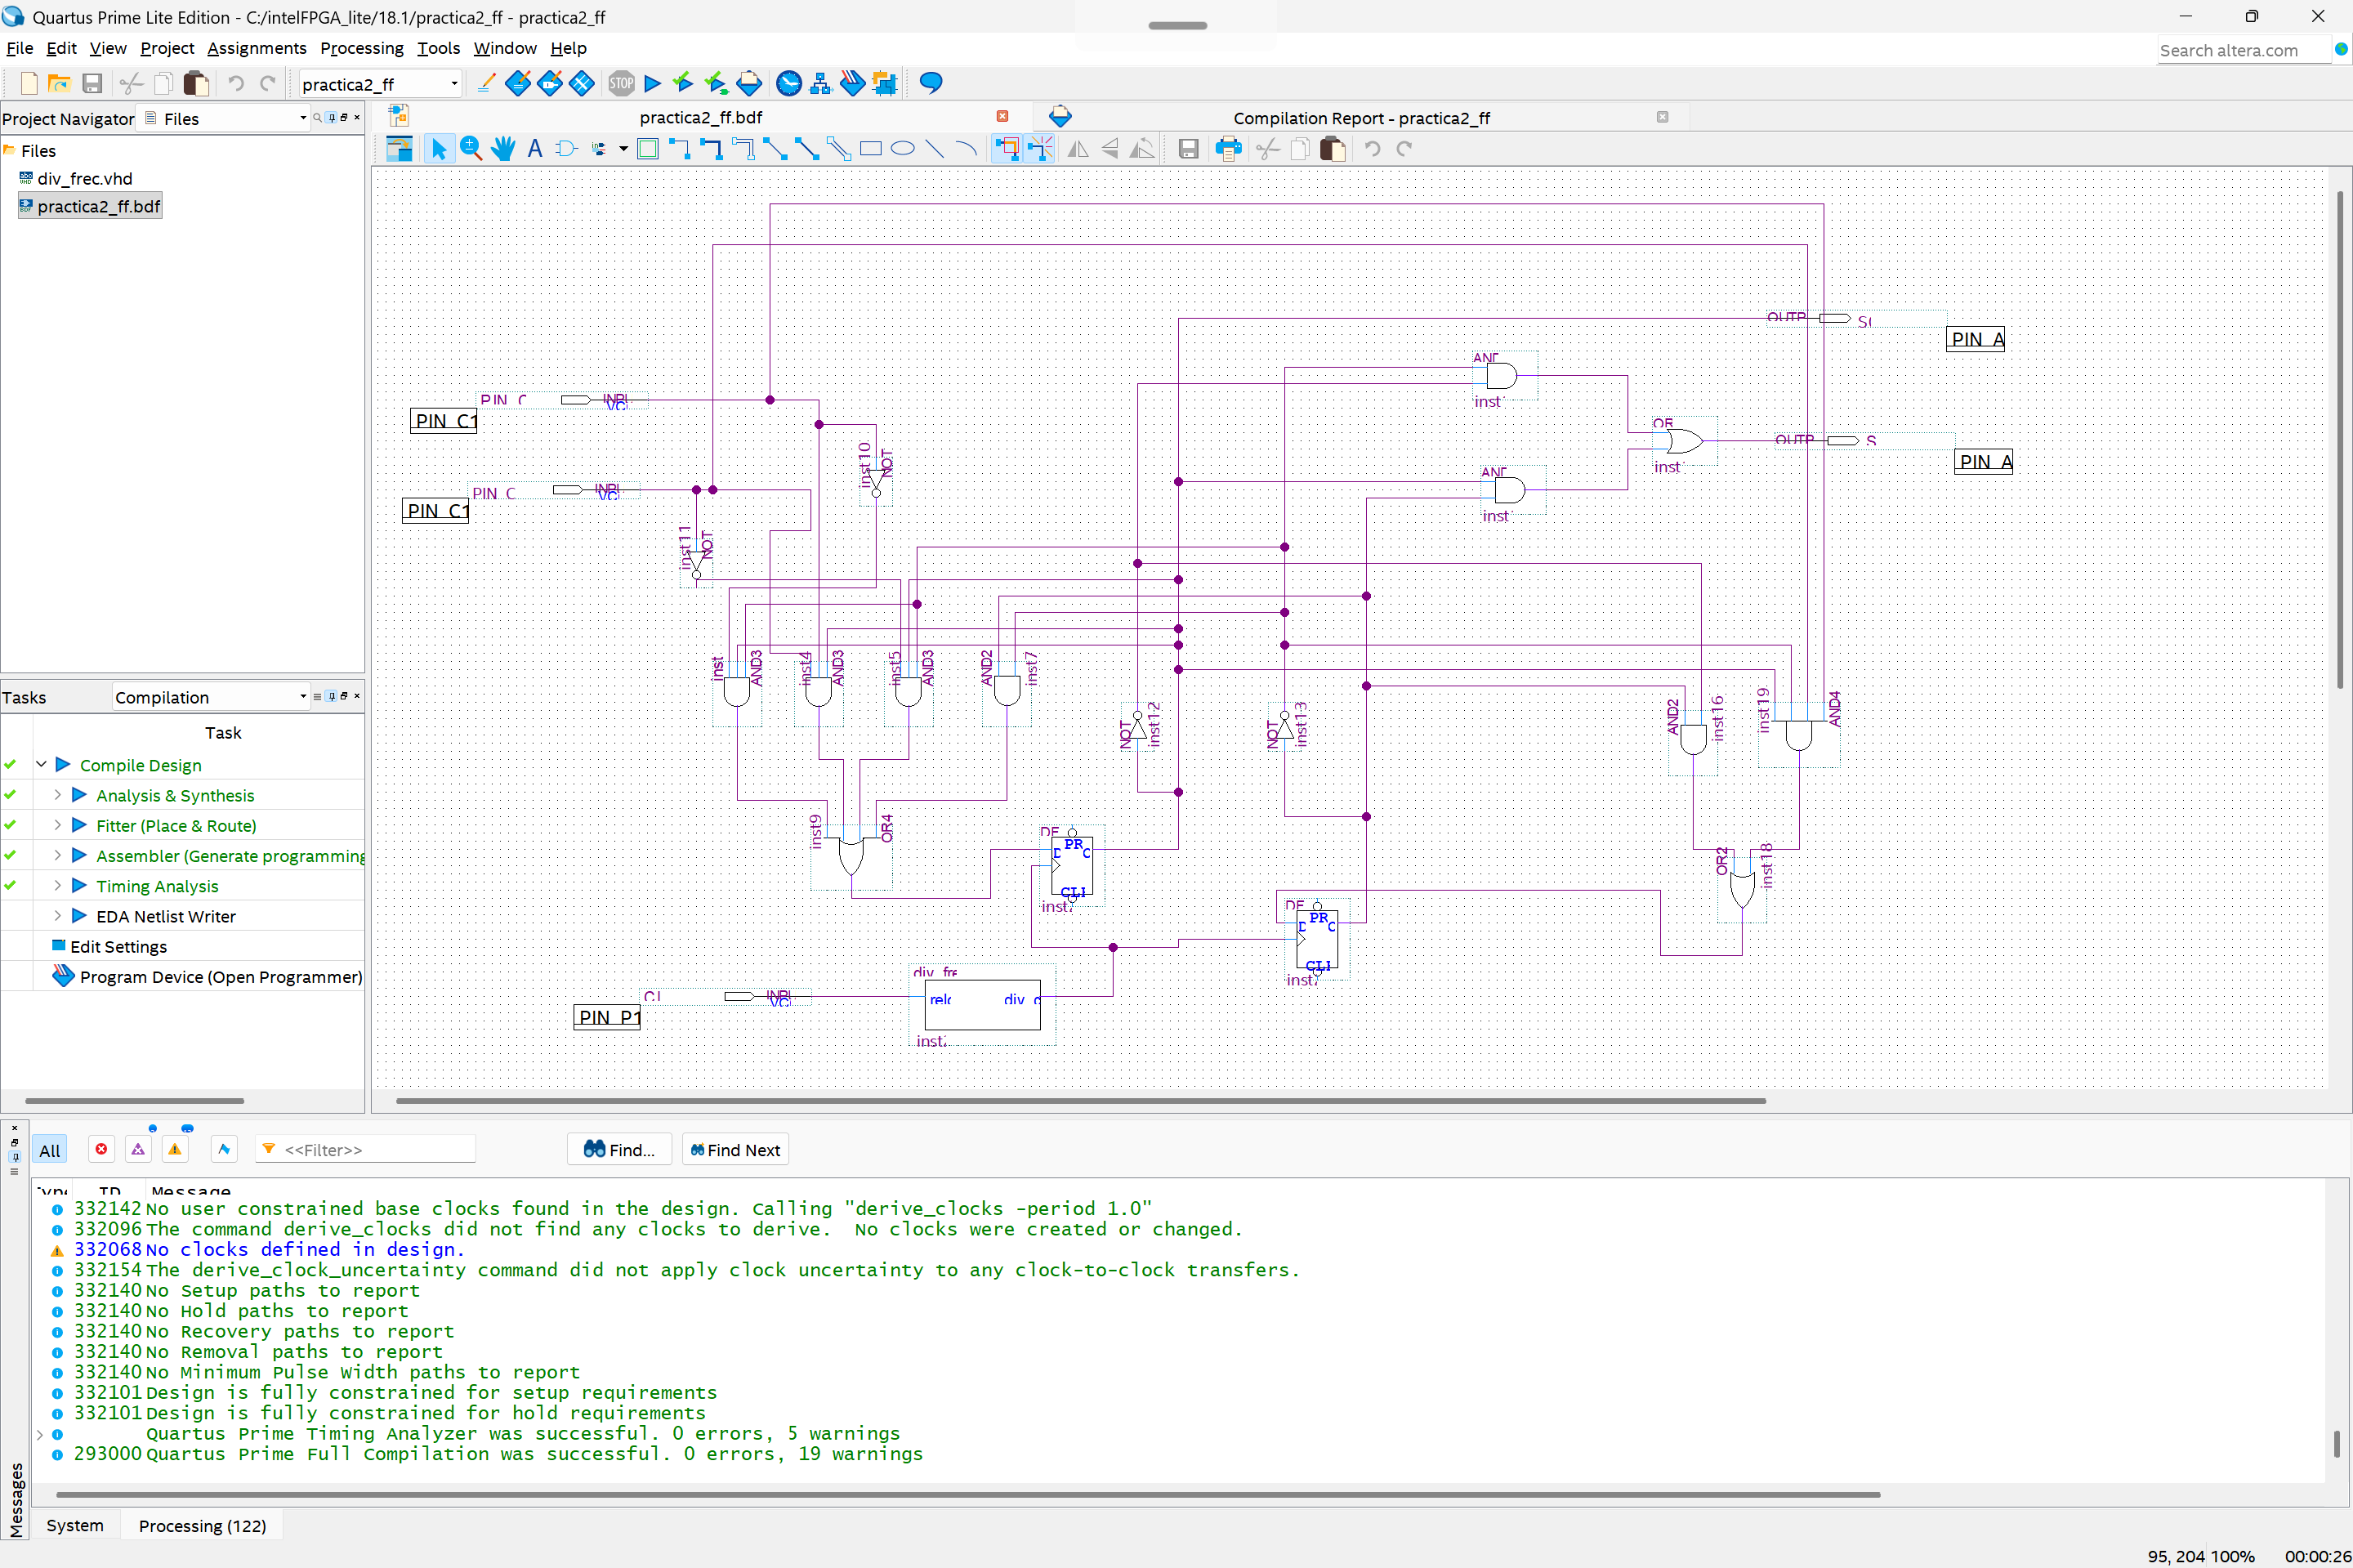
\includegraphics[width=\textwidth]{parte2-diagrama-logico-compilado.png}
  \caption{Esquemático compilado (\texttt{practica2\_ff.bdf}) en Quartus Prime,
    integrando \texttt{div\_frec} con la lógica de la máquina de estados.}
  \label{fig:diagrama-logico}
\end{figure}

\subsubsection{Implementación}

\todo[inline]{El manual pide implementar la máquina ``mediante VHDL'' (Parte II, paso 3);
  lo que se compiló fue un diagrama esquemático (\texttt{.bdf}) con compuertas
  individuales, no un módulo VHDL de la máquina de estados. Confirmar con la profesora si
  el esquemático es aceptado como equivalente o si además hay que escribir el código VHDL
  correspondiente a las ecuaciones \ref{eq:d1}-\ref{eq:s0} y agregarlo a
  \texttt{codigo/}.}

\subsubsection{Asignación de pines}

La asignación de entradas y salidas a los recursos físicos de la DE10-Lite, tomada del
\textit{Pin Planner} de Quartus, se muestra en la tabla \ref{tab:pines} y en la figura
\ref{fig:pin-planner}.

\begin{table}[H]
  \centering
  \begin{tabular}{llll}
    \toprule
    Señal & Dirección & Pin & Descripción \\
    \midrule
    CLK & Entrada & PIN\_P11 & Reloj de la tarjeta (50 MHz) \\
    PIN\_C10 & Entrada & PIN\_C10 & Entrada $X$ \\
    PIN\_C11 & Entrada & PIN\_C11 & Entrada $Y$ \\
    S0 & Salida & PIN\_A8 & Salida $S_0$ \\
    S1 & Salida & PIN\_A9 & Salida $S_1$ \\
    \bottomrule
  \end{tabular}
  \caption{Asignación de pines del proyecto \texttt{practica2\_ff}.}
  \label{tab:pines}
\end{table}

\begin{figure}[H]
  \centering
  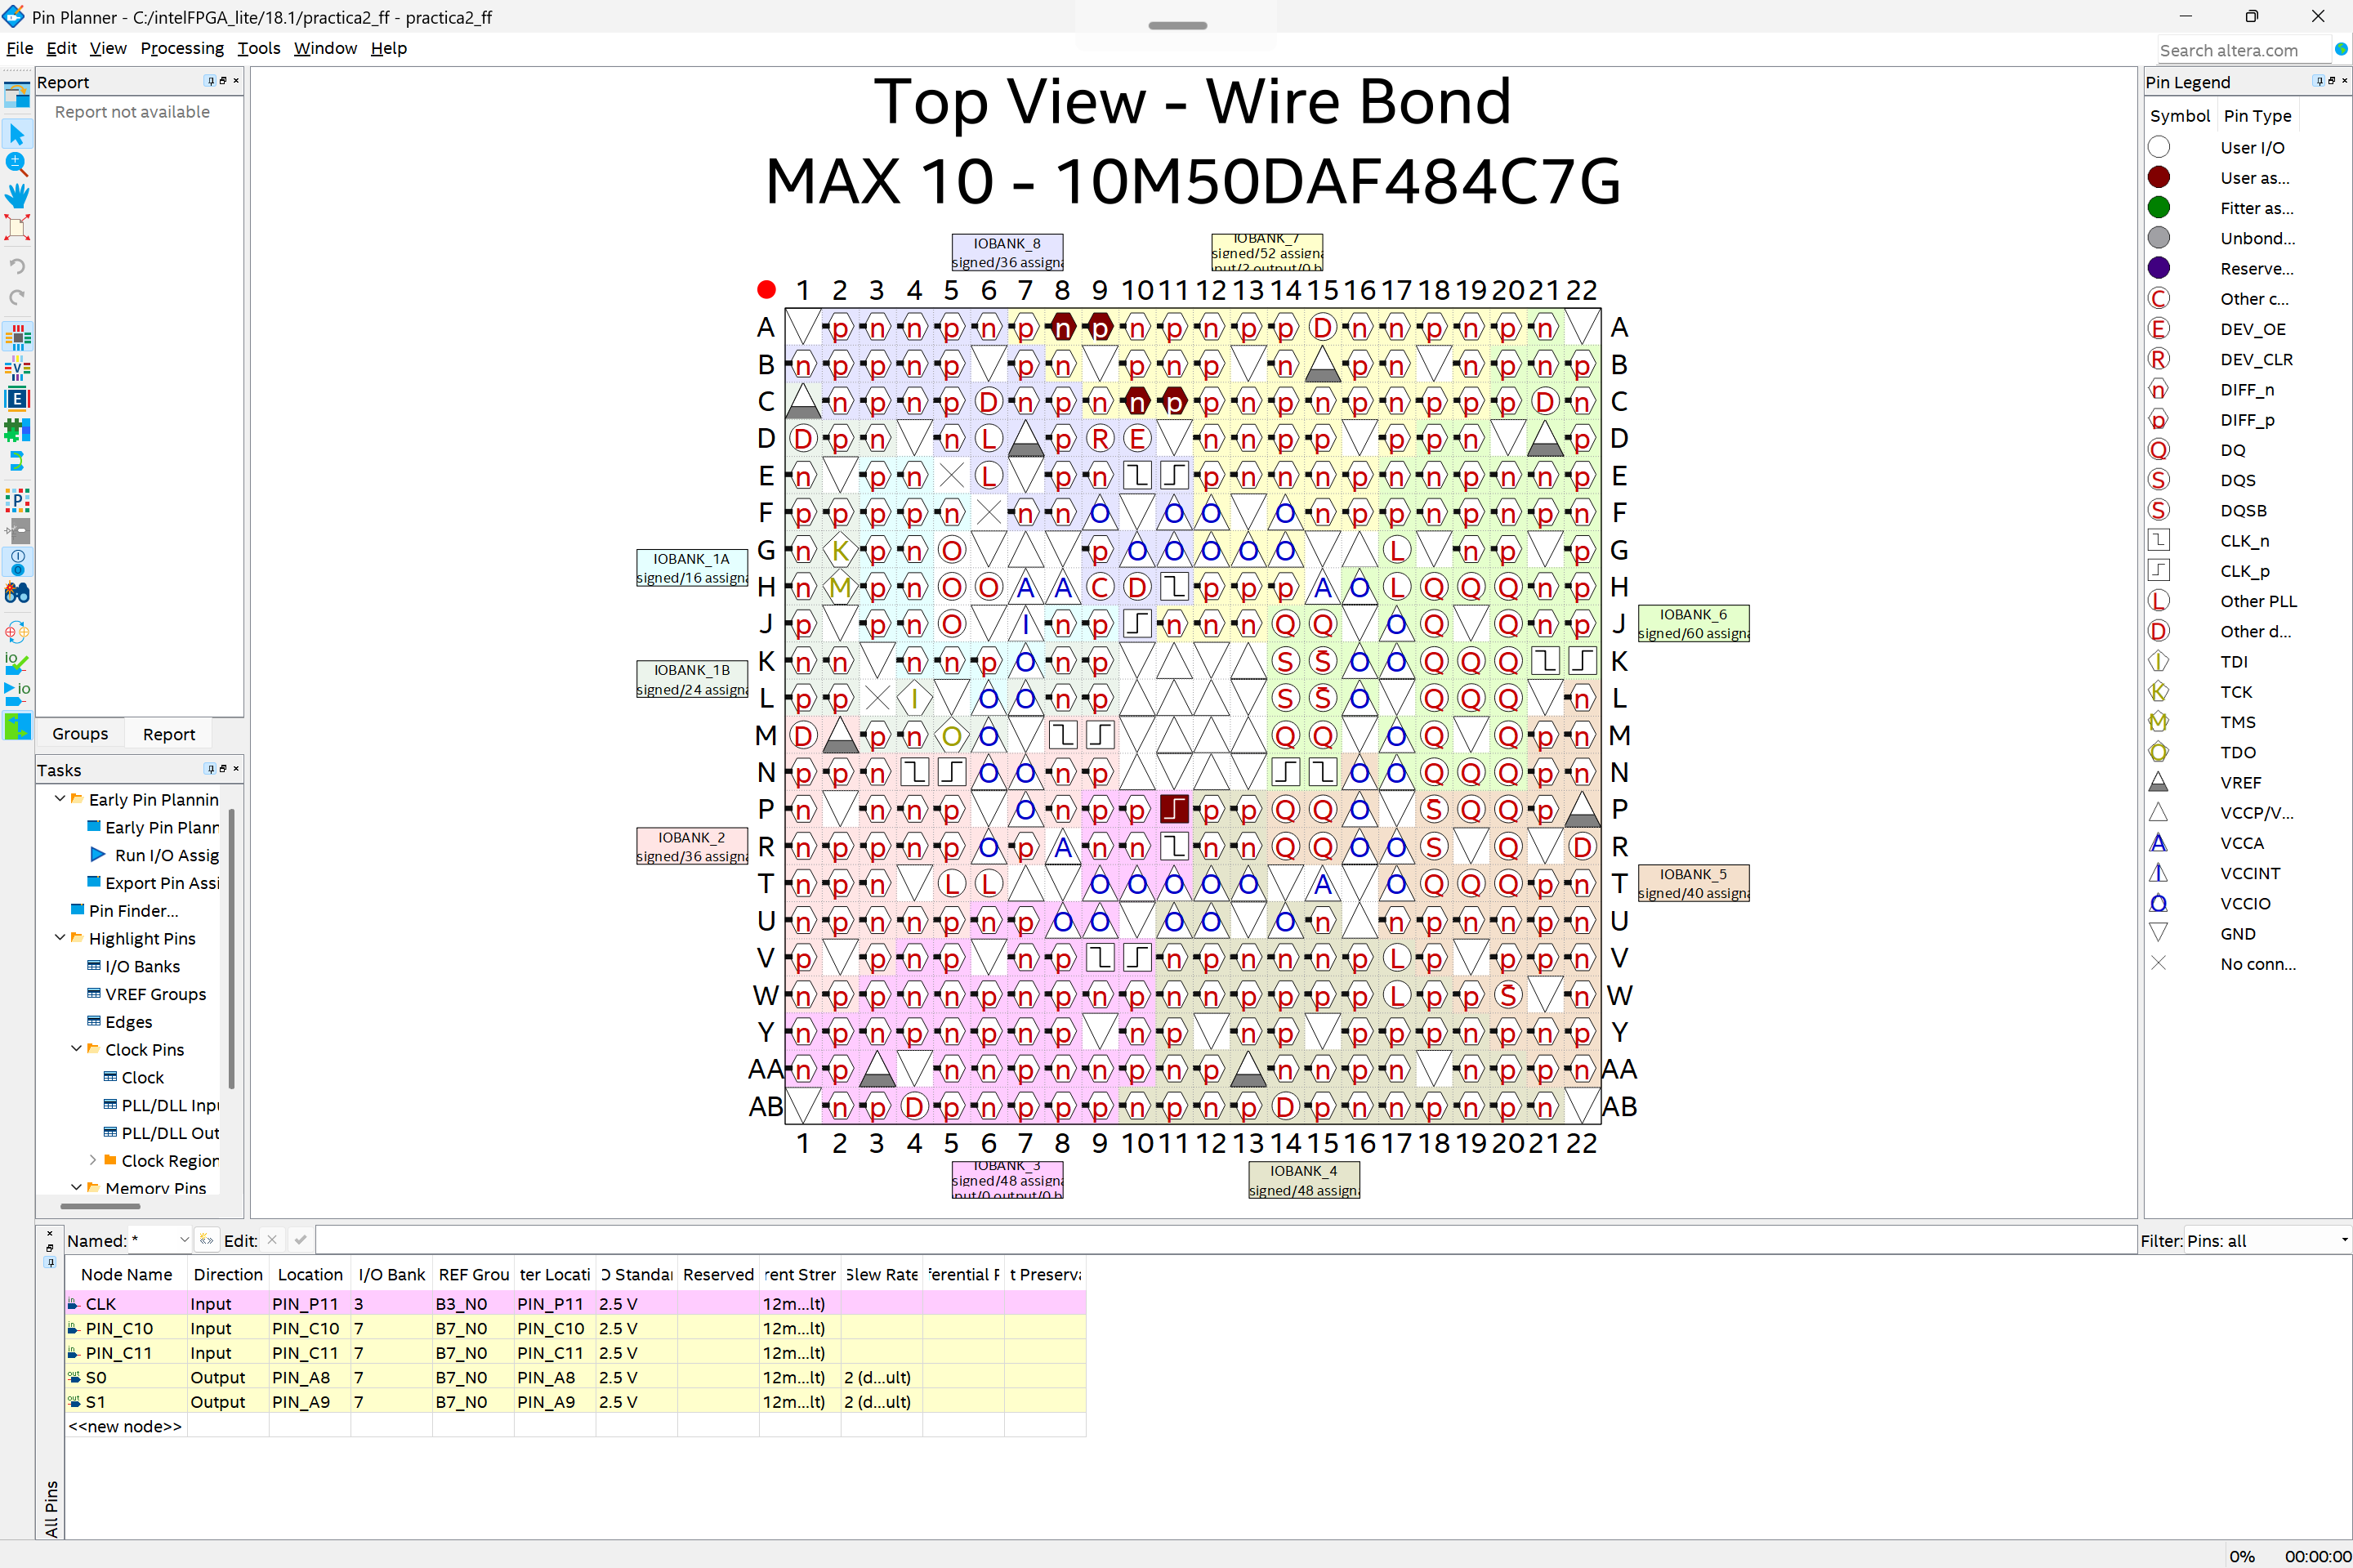
\includegraphics[width=\textwidth]{parte2-pin-planner.png}
  \caption{\textit{Pin Planner} de Quartus Prime mostrando el dispositivo
    (MAX 10 -- 10M50DAF484C7G) y la tabla de asignación de pines.}
  \label{fig:pin-planner}
\end{figure}

\todo[inline]{Documentar a qué recurso físico de la tarjeta corresponde cada pin (por
  ejemplo, \texttt{PIN\_C10}/\texttt{PIN\_C11} a los interruptores SW usados como $X$/$Y$,
  y \texttt{PIN\_A8}/\texttt{PIN\_A9} a los LEDs usados como $S_0$/$S_1$), según la hoja
  de pines oficial de la DE10-Lite.}

\subsubsection{Compilación y programación de la FPGA}

El proyecto compiló sin errores: el reporte de compilación de la figura
\ref{fig:diagrama-logico} indica ``\textit{Quartus Prime Full Compilation was
successful. 0 errors, 19 warnings}''. La FPGA se programó y se comprobó su
funcionamiento físicamente, como se muestra en la figura \ref{fig:tarjeta}.

\todo[inline]{Revisar y, si aplica, describir en el reporte a qué se deben las 19
  advertencias de compilación (\textit{warnings}); usualmente no impiden el
  funcionamiento pero conviene documentarlas.}

\subsubsection{Comprobación experimental}

Se tomaron fotografías de la tarjeta DE10-Lite programada con distintas combinaciones de
las entradas $X$, $Y$ (figura \ref{fig:tarjeta}).

\begin{figure}[H]
  \centering
  \begin{minipage}{0.32\textwidth}\centering
    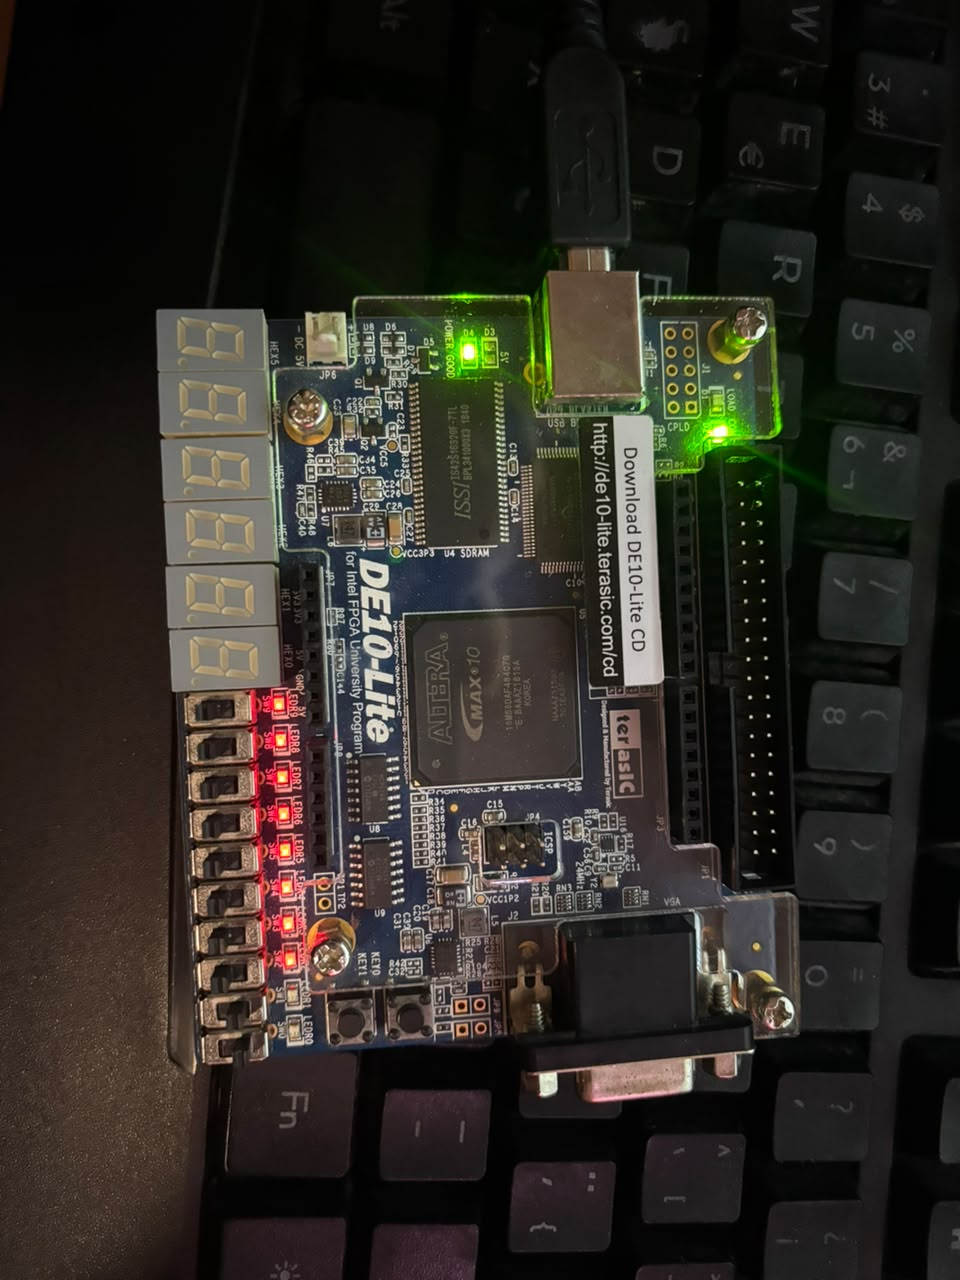
\includegraphics[width=\textwidth]{parte2-00.jpeg}\\
    $XY=00$
  \end{minipage}\hfill
  \begin{minipage}{0.32\textwidth}\centering
    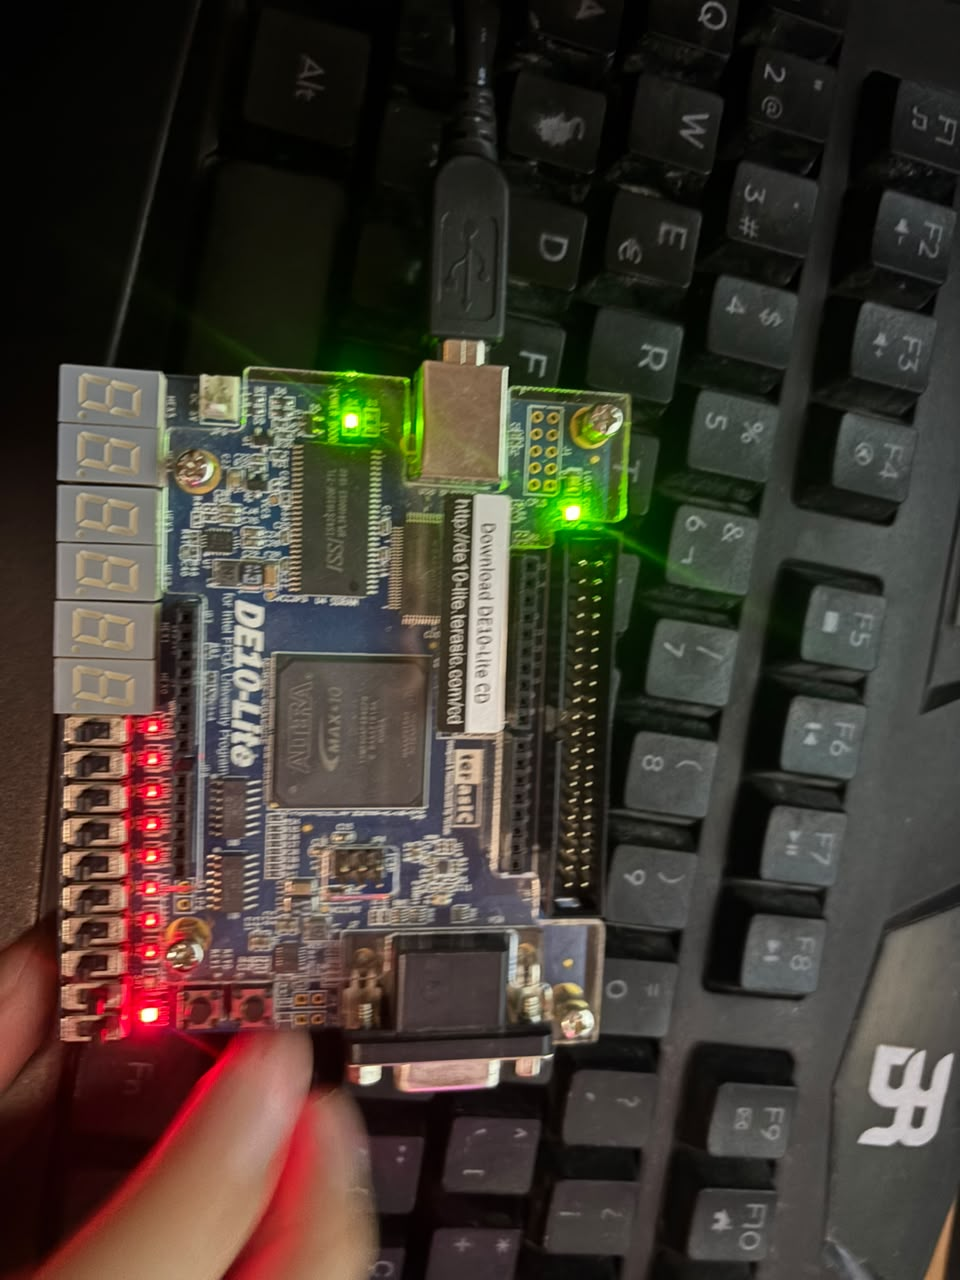
\includegraphics[width=\textwidth]{parte2-01-.jpeg}\\
    $XY=01$
  \end{minipage}\hfill
  \begin{minipage}{0.32\textwidth}\centering
    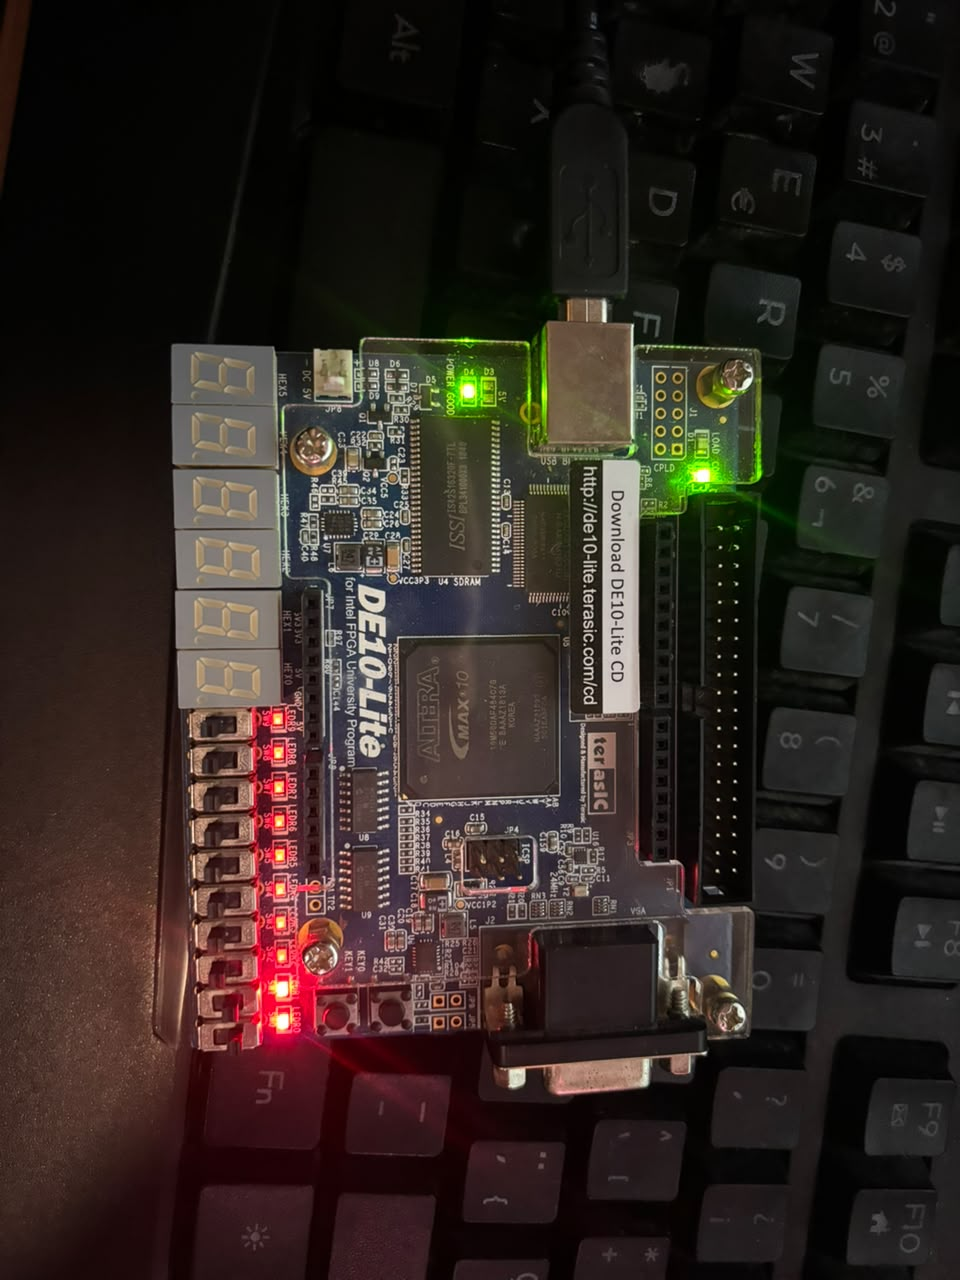
\includegraphics[width=\textwidth]{parte2-11.jpeg}\\
    $XY=11$
  \end{minipage}
  \caption{Tarjeta DE10-Lite programada, con los interruptores en las combinaciones
    $XY=00$, $01$ y $11$.}
  \label{fig:tarjeta}
\end{figure}

\todo[inline]{Las fotografías confirman que la tarjeta quedó programada y encendida
  (LEDs y \textit{power good} activos), pero por el ángulo/iluminación no se alcanza a
  leer con certeza qué LEDs específicos codifican $S_1S_0$ en cada captura. Completar:
  (1) describir qué LEDs/recursos muestran el estado y la salida en cada foto, (2)
  agregar la combinación $XY=10$ que falta, y (3) para cada captura, indicar en qué
  estado (EST0-EST3) se encontraba la máquina y compararlo contra la tabla
  \ref{tab:transiciones}.}

\section{Análisis de resultados}

De acuerdo con las secciones anteriores, el diseño de la Parte I (tabla de transiciones,
mapas de Karnaugh y ecuaciones \ref{eq:d1}-\ref{eq:s0}) se implementó y compiló sin
errores en Quartus, y la tarjeta fue programada y responde a los interruptores de
entrada. \todo[inline]{Falta la comparación explícita, transición por transición, entre
  el comportamiento observado en la FPGA (figura \ref{fig:tarjeta}, y las combinaciones
  que falten por capturar) y lo previsto en la tabla \ref{tab:transiciones} de la Parte
  I, señalando si coinciden o si se encontró alguna discrepancia.}

\section{Conclusiones individuales}

\subsection{Omar Alfonso Zendejas Labias}

\todo[inline]{Redactar la conclusión individual una vez concluidas ambas partes de la
  práctica.}

\subsection{Emiliano García Olvera}

\todo[inline]{Redactar la conclusión individual una vez concluidas ambas partes de la
  práctica.}

\begin{thebibliography}{9}
\bibitem{savage} J. Savage Carmona, G. Vázquez y N. E. Chávez Rodríguez,
  \emph{Diseño de microprocesadores}. Ciudad de México, México: Facultad de Ingeniería,
  Universidad Nacional Autónoma de México, 2017. [En línea]. Disponible:
  \url{http://profesores.fi-b.unam.mx/luist/archivos/MicroprocesadoresSavage.pdf}
\end{thebibliography}

\end{document}
